\begin{figure*}[t]
\centering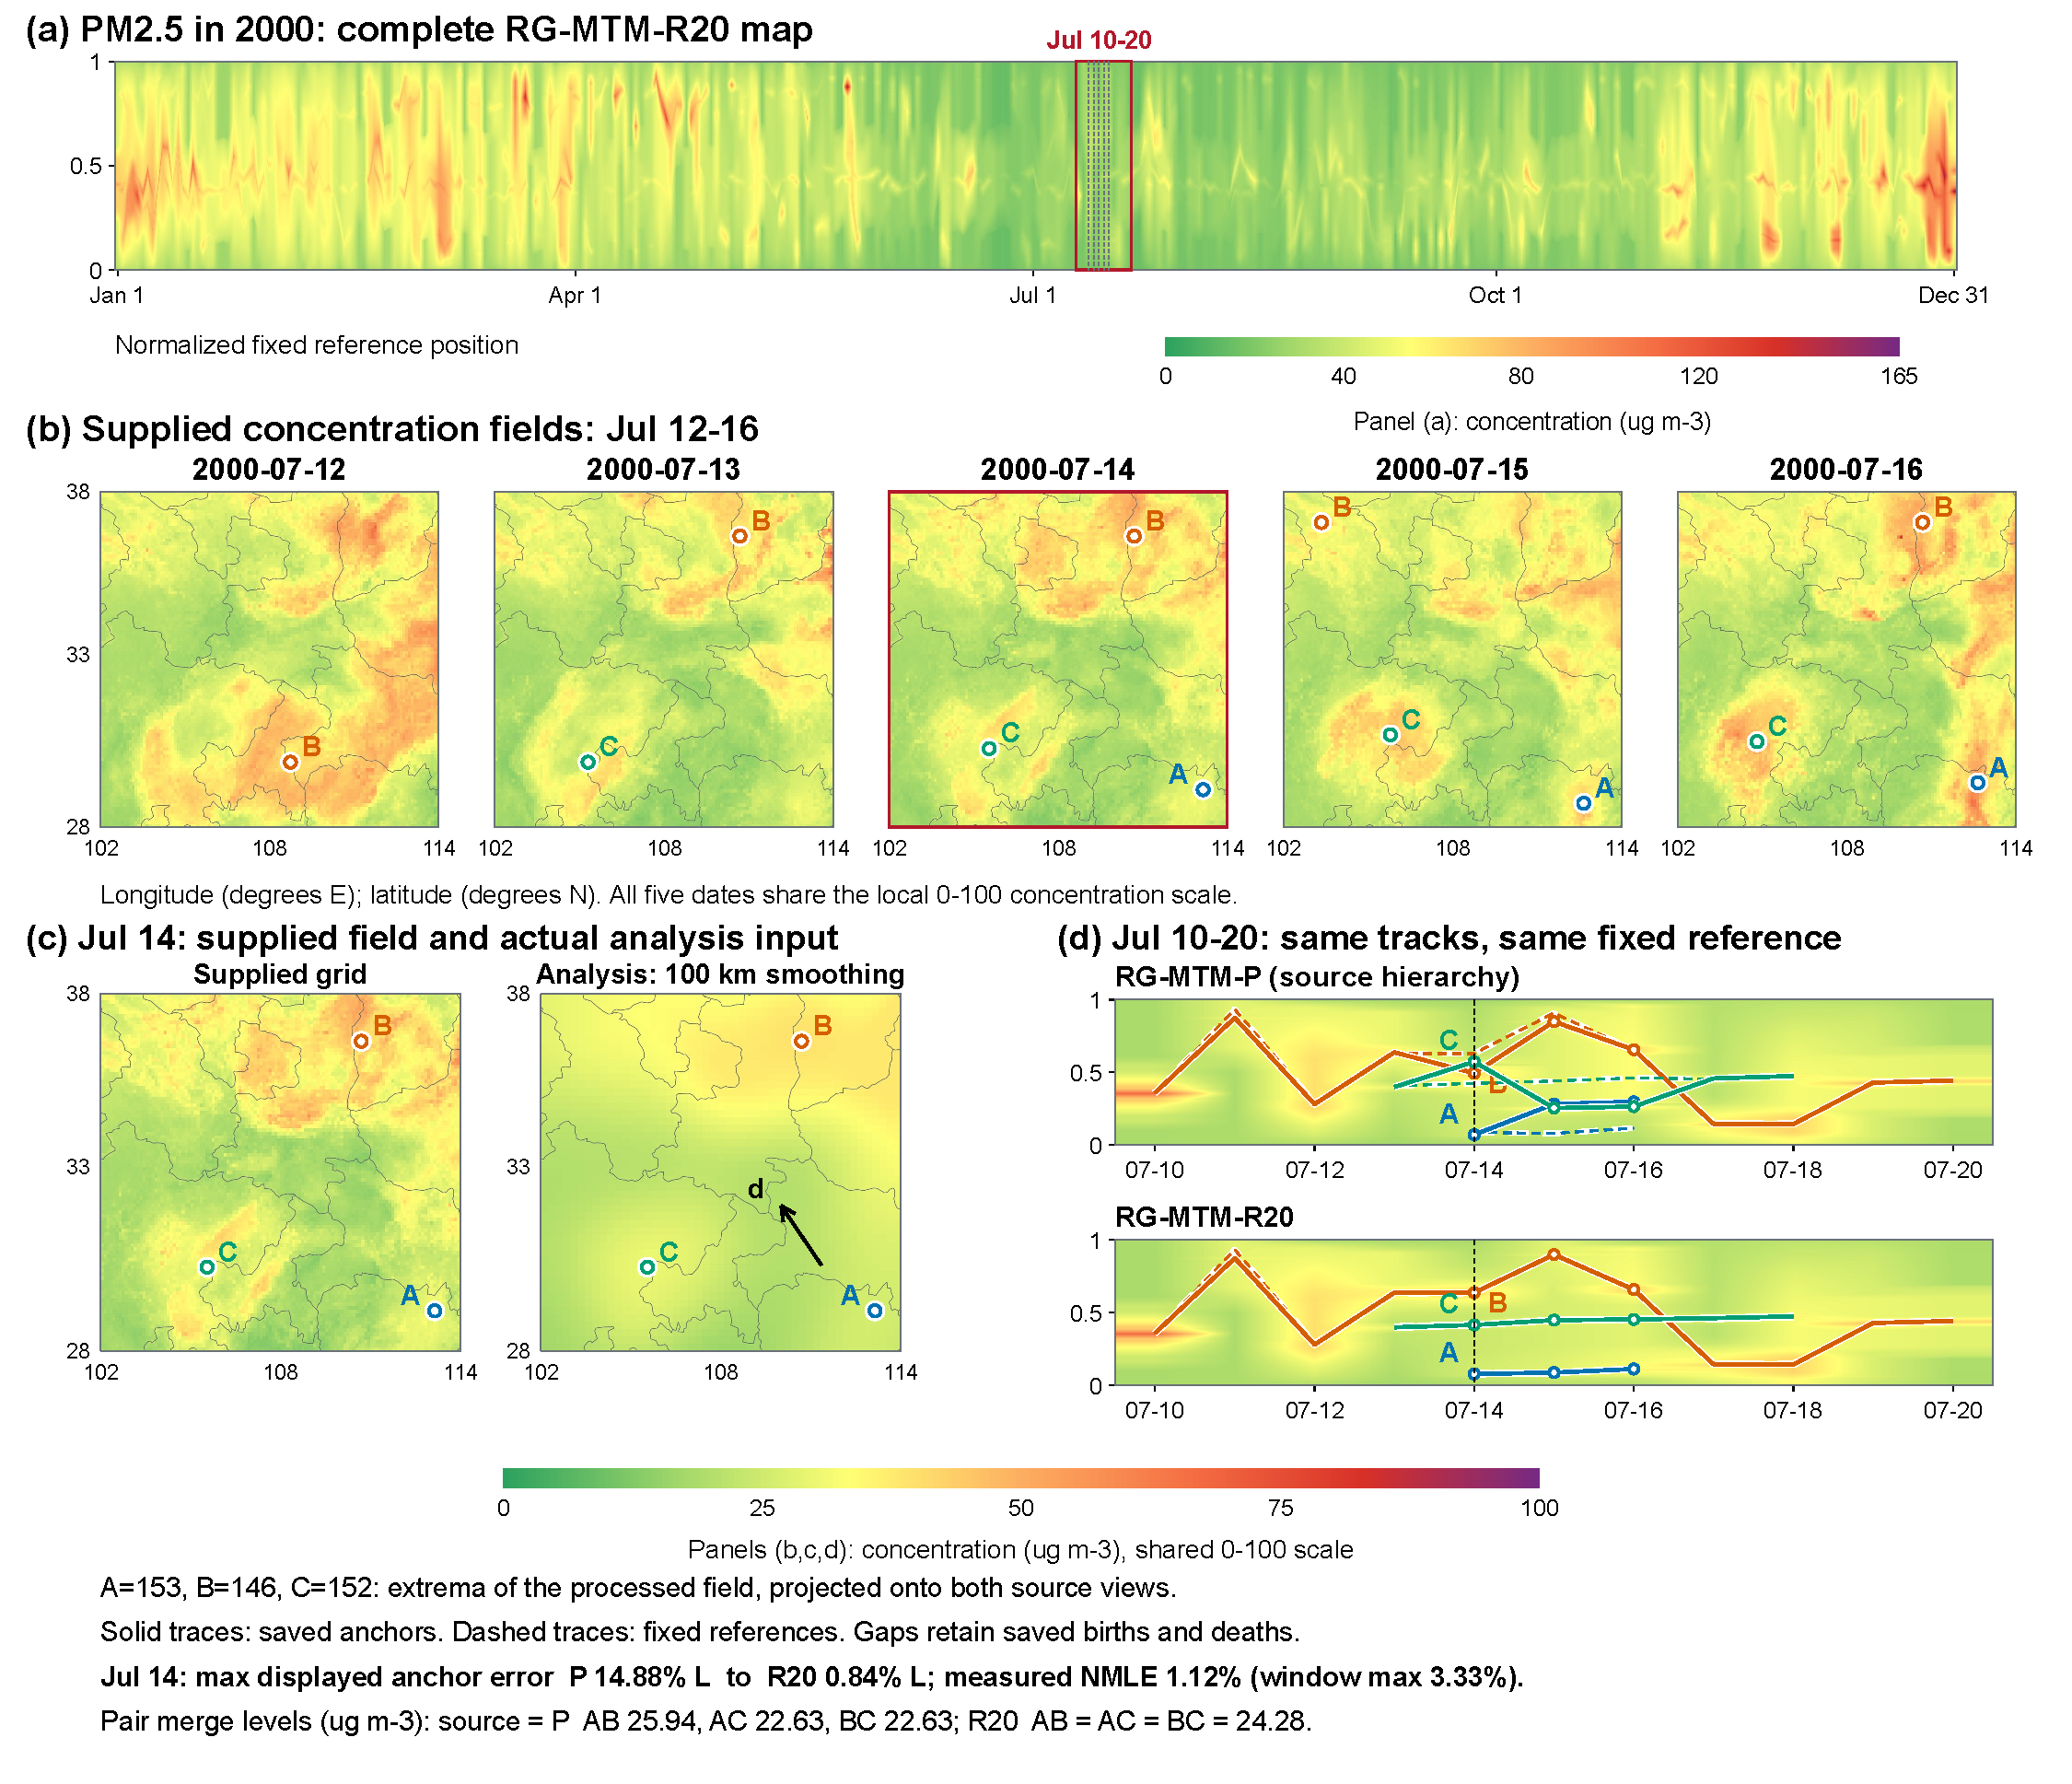
\includegraphics[width=\textwidth]{figures/Fig13.pdf}
\caption{PM2.5: complete-year context and a source-linked July case. (a) All 366 R20 profiles with July 10--20 outlined. (b) Supplied concentration fields for July 12--16, with geographic context from Natural Earth~\cite{NaturalEarth:Admin1}. (c) July 14 supplied and processed fields; markers show the same processed extrema $A=153,B=146,C=152$, and $d$ is the fixed annual reference direction. (d) Complete P/R20 profiles over July 10--20, with solid saved anchors and dashed fixed references. Tracks retain their saved births and deaths. Panel (a) uses 0--165\,$\mu$g\,m$^{-3}$; panels (b)--(d) share 0--100\,$\mu$g\,m$^{-3}$ without per-date rescaling. At July 14, maximum displayed-anchor displacement falls from 14.88\% to 0.84\% of $L$, at 1.12\% measured NMLE; the window's maximum NMLE is 3.33\%. This is a selected mechanism witness, not a claim of annual motion improvement. Display interpolation preserves every saved profile.}
\label{fig:pm25_case}
\end{figure*}
